\chapter{Experiments\label{cha:chapter4}}
\hspace*{1em}This chapter details the experiments conducted in the context of this thesis.
We evaluate the proposed methods on three image classification datasets:
MNIST \cite{lecun2010mnist},
CIFAR-10 \cite{krizhevsky2009learning},
and Imagenette \cite{DBLP:journals/information/HowardG20}, which is a subset of 10 easily classified classes from the ImageNet dataset.
First, we provide an overview of the experimental setup.
We then present the results of the gradient ratio thresholding method, as detailed in \cref{sec:nestedquantizationlayer},
followed by the results of the custom loss terms discussed in \cref{sec:customloss}.

% ------------------------------------------------------------
% ----------------------- Setup ----------------------- 
% ------------------------------------------------------------

\section{Experimental Setup}
\label{sec:setup}
\hspace*{1em}\textbf{Software and Hardware Setup.} As briefly mentioned in \cref{sec:nestedquantizationlayer},
our custom methods are implemented in TensorFlow.
Specifically, we used TensorFlow version 2.11.0, running on Python 3.10.14. 
All experiments are conducted on a server equipped with two NVIDIA A40 GPUs, 
each with 48 GB of memory, running on CUDA 11.4 and driver version 470.256.02.

\textbf{Experiment Networks.} 
For simplicity and tractability, we define custom networks for each dataset.
For MNIST, we use a small network consisting of two dense layers, 
each adjusted to incorporate nested quantization layers for both weights and biases. 
For CIFAR-10, we use a convolutional network with three blocks of convolutional layers, 
each adjusted to incorporate nested quantization layers for both kernels and biases.
These are followed by two dense layers.
The Imagenette model is a ResNet-inspired architecture,
featuring an initial quantized convolutional block followed by four stages of residual blocks. 
Each residual block incorporates the adjusted convolutional layers with nested quantization 
for both kernels and biases. For the experimentation with custom loss terms, 
we use equivalent networks without the nested quantization layer logic.

\textbf{Baseline Hyperparameters and Initialization.} Using the hyperparameters described in \cref{tab:hyperparameters}, 
each network optimizes its parameters using the Adam optimizer and the sparse categorical cross-entropy loss function. 
Weights and biases are initialized with random normal values, 
while scale factors are initialized with very small constant values for all cases. 
Scale factors are constrained to be positive and non-zero to avoid numerical issues during division. 
An example implementation for reproducing these networks is available at the following GitHub Gist: INSERT LINK

\begin{table}[t!]
  \centering
  \caption{Network Settings for Different Datasets}
  \label{tab:hyperparameters}
  \begin{tabular}{lccc}
      \toprule
      \textbf{Hyperparameter}     & \textbf{MNIST} & \textbf{CIFAR-10} & \textbf{Imagenette} \\ 
      \midrule
      Learning Rate               & 0.0001            & 0.0001              & 0.001              \\ 
      Batch Size                  & 32                & 128                 & 64                 \\ 
      Epochs                      & 100               & 100                 & 100                \\ 
      Seeds for Reproducibility   & 1-3,42,1337     & 1-3,42,1337       & 1-3,42,1337                 \\ 
      \bottomrule
  \end{tabular}
\end{table}
% ------------------------------------------------------------
% ----------------------- Pareto stuff ----------------------- 
% ------------------------------------------------------------

\section{Optimal Thresholds for Nested Quantization Layers}
\label{sec:paretofronts}
\hspace*{1em}For the nested quantization layer method, we evaluate the results across different thresholds \( \lambda \)
for both dense and convolutional layers. The first subsection presents results for fully connected layers trained on MNIST,
while the second subsection focuses on convolutional layers trained on CIFAR-10 and Imagenette.

\subsection{Fully Connected Layers}
\label{subsec:paretofrontsdense}
\hspace*{1em}As mentioned earlier, we use a small network with two dense layers trained on the MNIST dataset. 
These two dense layers have weight matrices \( W_1 \) and \( W_2 \),
along with bias vectors \( b_1 \) and \( b_2 \).
We examine three scenarios:
applying the scale factor row-wise, 
column-wise, and as a single scalar for the entire weight matrix.
For all scenarios, a scalar scale factor is used for each bias vector. 
The configurations are shown in \cref{tab:scalefactorgranularitydense}.

\begin{table}[b!]
  \centering
  \caption{Scale Factor Granularity}
  \label{tab:scalefactorgranularitydense}
  \begin{tabular}{lccc}
    \toprule
    \textbf{Parameter}             & \textbf{Row-wise}       & \textbf{Column-wise}       & \textbf{Scalar}       \\ 
    \midrule
    \( W_1 \) \( (784, 128) \) & \( s \) \( (784, 1) \)        & \( s \) \( (1, 128) \)           & \( s \) \( (1, 1) \)         \\ 
    \( b_1 \) \( (128, 1) \)   & \( s \) \( (1, 1) \)          & \( s \) \( (1, 1) \)             & \( s \) \( (1, 1) \)         \\ 
    \( W_2 \) \( (128, 10) \)  & \( s \) \( (128, 1) \)        & \( s \) \( (1, 10) \)            & \( s \) \( (1, 1) \)         \\ 
    \( b_2 \) \( (10, 1) \)    & \( s \) \( (1, 1) \)          & \( s \) \( (1, 1) \)             & \( s \) \( (1, 1) \)         \\ 
    \bottomrule
  \end{tabular}
  \vspace{0.5em}
%  \caption*{\footnotesize Note: \( (,) \) represents a scalar value — scalars technically have no dimensions.}
\end{table}


The experiments have demonstrated that the optimal quantization is observed for a penalthy threshold of 
\( \lambda = 1e-10 \) across all three scenarios.
This conclusion is based on Pareto front plots in \cref{fig:pareto-mnist-dense},
which illustrate the trade-off between accuracy loss and quantization.
We see that, for all scenarios, 
the number of unique integer values after quantization, 
aggregated across all parameters of the two dense layers, reaches its lowest point at \( \lambda = 1e-10 \)
without significantly degrading the accuracy.

As an example, the actual integer values after quantization for the rowwise scenario is 
depicted in \cref{fig:quantization_results_1e-10_dense} for all four parameters separately.
While the total number of unique values is only \( 24 \), the range spans from \( -12 \) to \( 11 \).
This means that \( 5 \) bits are sufficient to represent the quantized values in the resulting layers, 
as \( \lceil \log_2(24) \rceil = 5 \), covering all 24 unique values within the range. 
This can even be further reduced using compression techniques like Huffman coding \cite{4051119}, 
considering the concentration of values around 0 in the distributions of weight quantizations.

Interestingly, as depicted in \cref{fig:val-losses-over-epochs-dense}, 
the validation loss for \( \lambda = 1e-10 \) 
consistently remains lower than the baseline  \( \lambda = 0.0 \) throughout the training process.
At the same time, the validation accuracy, shown in \cref{fig:val-accs-over-epochs-dense}
remains almost identical to the baseline. This indicates that the penalty threshold
\( \lambda = 1e-10 \) 
not only preserves classification accuracy
but also improves generalization in terms of loss,
making the model more confident in its predictions.

In terms of quantization granularity, we see that a scalar scaling factor applied to 
weights produces the worst results compared to row-wise and column-wise granularity.
This is evident from the steeper accuracy degradation and greater loss increase for
 \( \lambda = 1e-8\), as shown in \cref{fig:val-accs-over-epochs-dense} and
\cref{fig:val-losses-over-epochs-dense}.
The poor performance of the scalar scaling factor suggests 
that layer-wise quantization, 
which it represents, 
is too coarse to account for the variability in parameter distributions within a layer.
Therefore, finer granularities, such as row-wise or column-wise scaling, 
are more suitable candidates for optimal quantization granularity of dense layers.

\begin{figure}[t!]
  \centering
  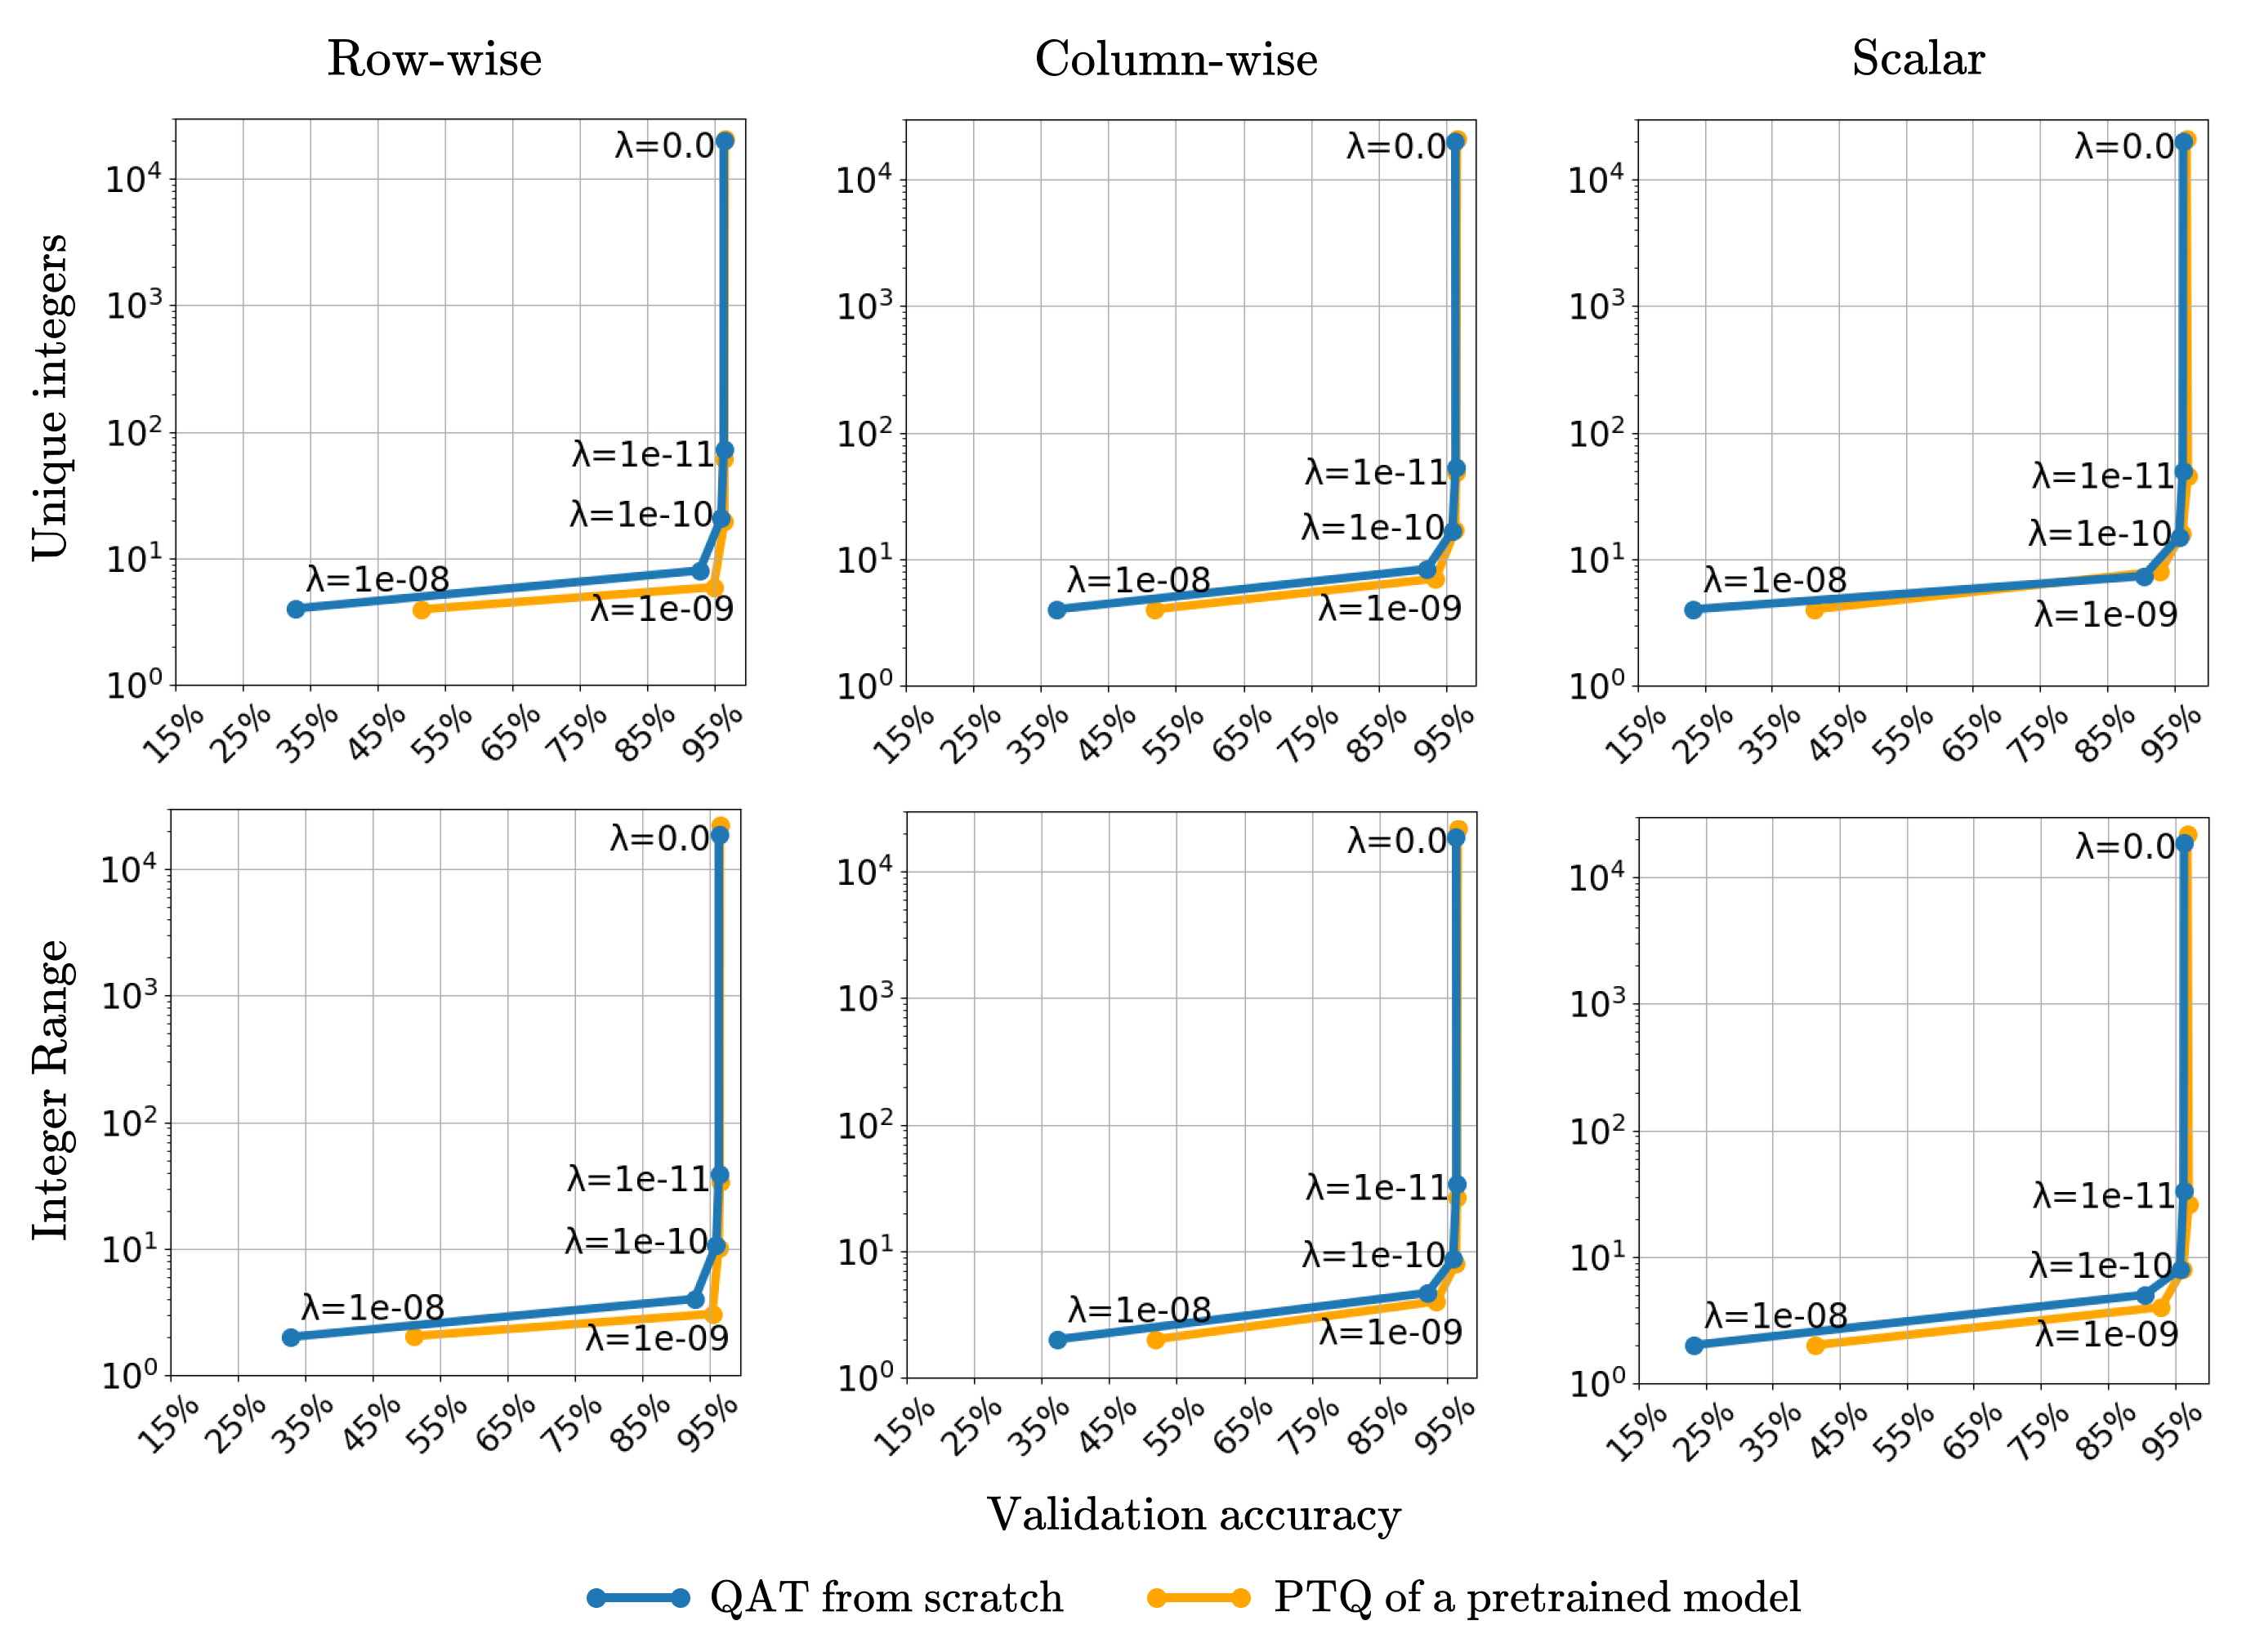
\includegraphics[width=14cm]{pareto-mnist-dense.png}
  \caption{Impact of quantization on accuracy for different \( \lambda \). Rowwise (left), columnwise (middle) and scalar (right) scaling factors applied to weights of dense layers, with a scalar scaling factor — to biases.}
  \label{fig:pareto-mnist-dense}
\end{figure}


\begin{figure}[t!]
  \centering
  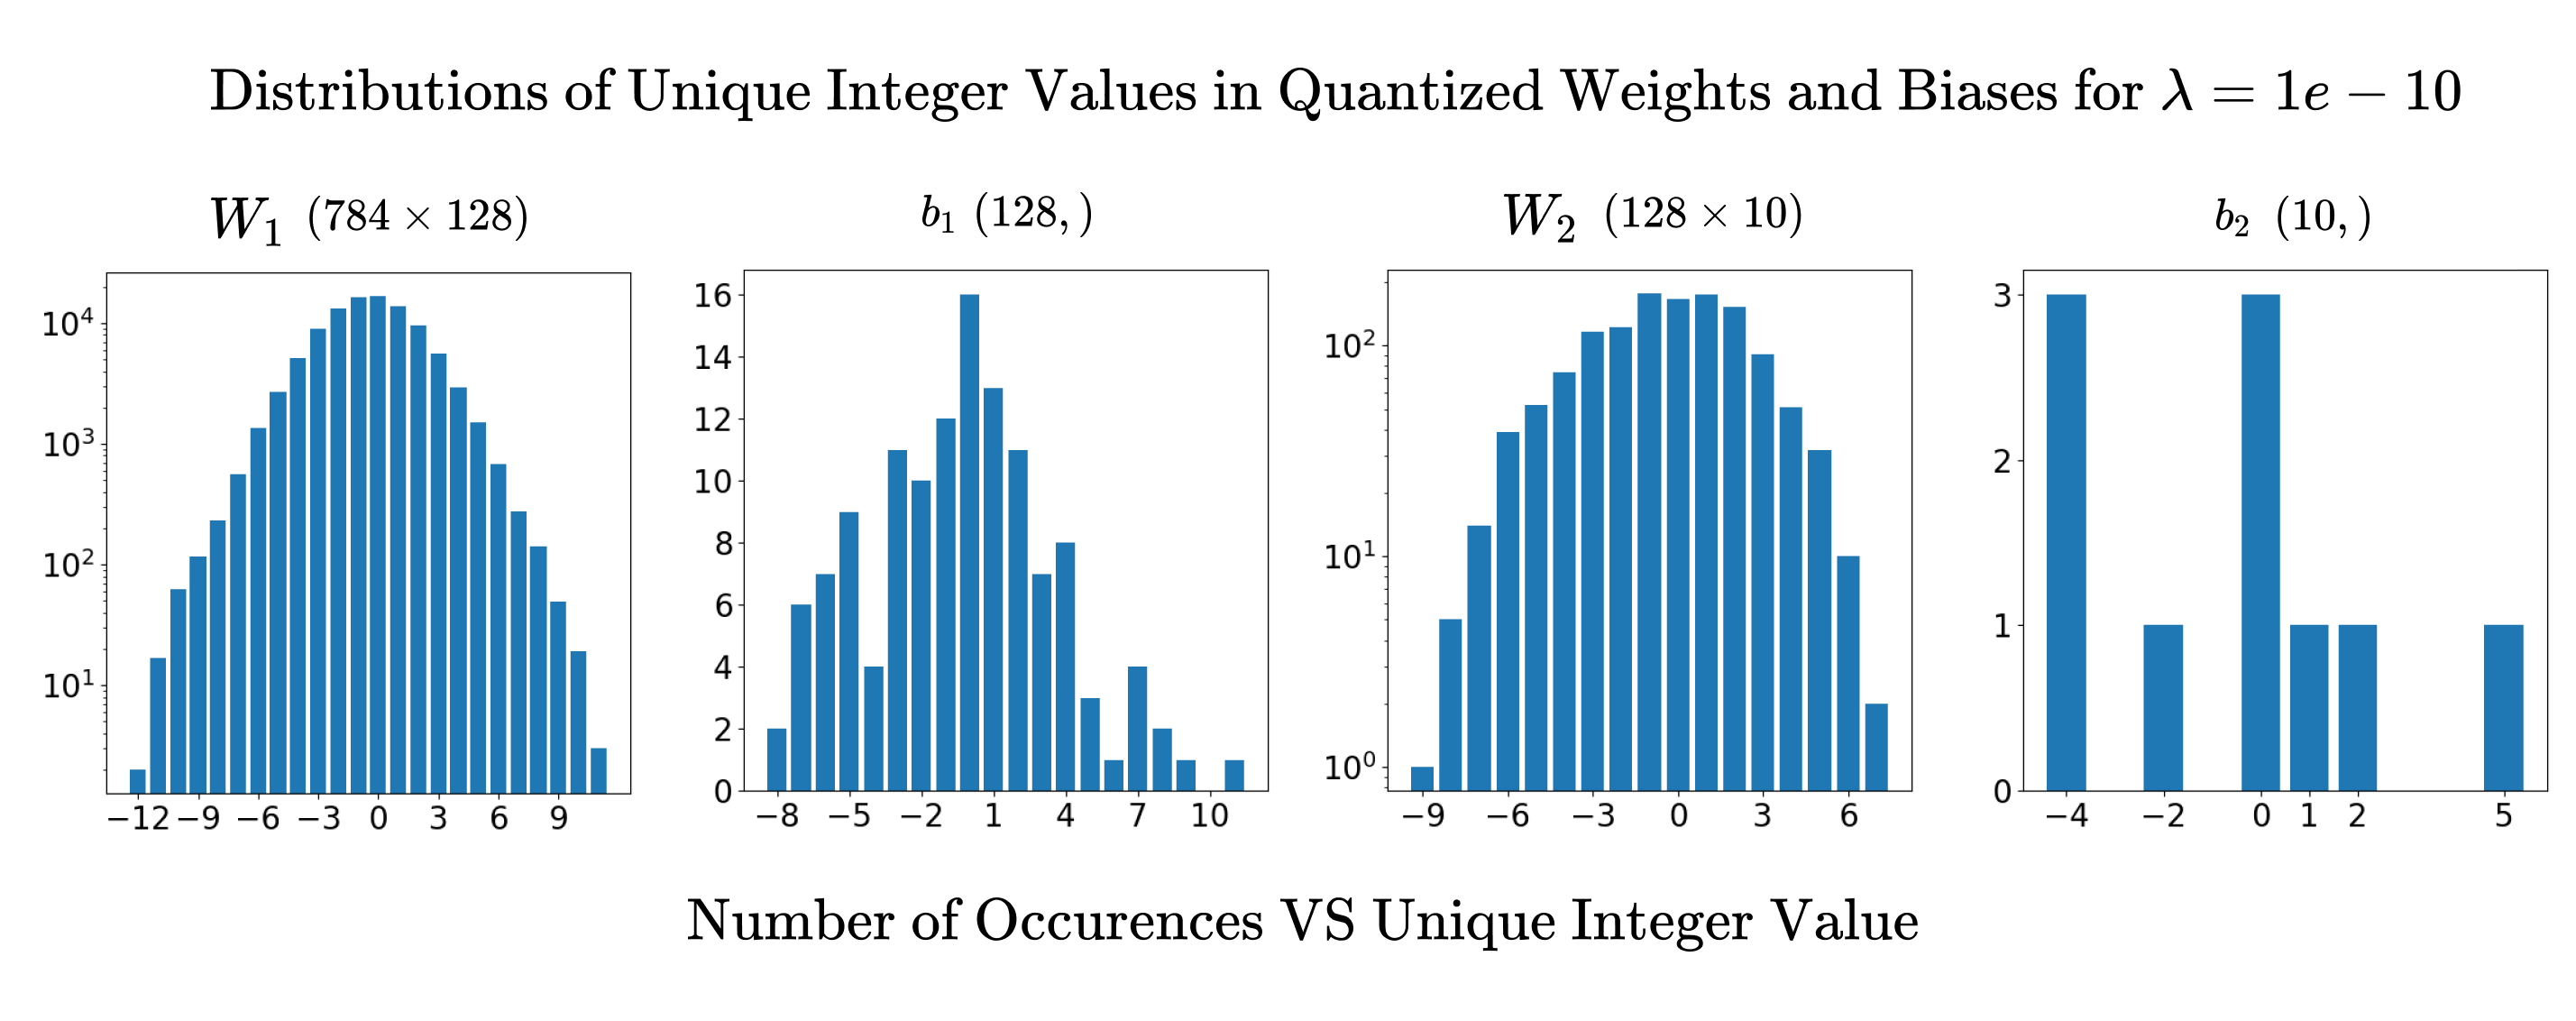
\includegraphics[width=14cm]{quantization_results_1e-10_dense.png}
  \caption{Rowwise scaling factors applied to the weights of dense layers, with a scalar scaling factor — to the biases.}
  \label{fig:quantization_results_1e-10_dense}
\end{figure}


\begin{figure}[b!]
  \centering
  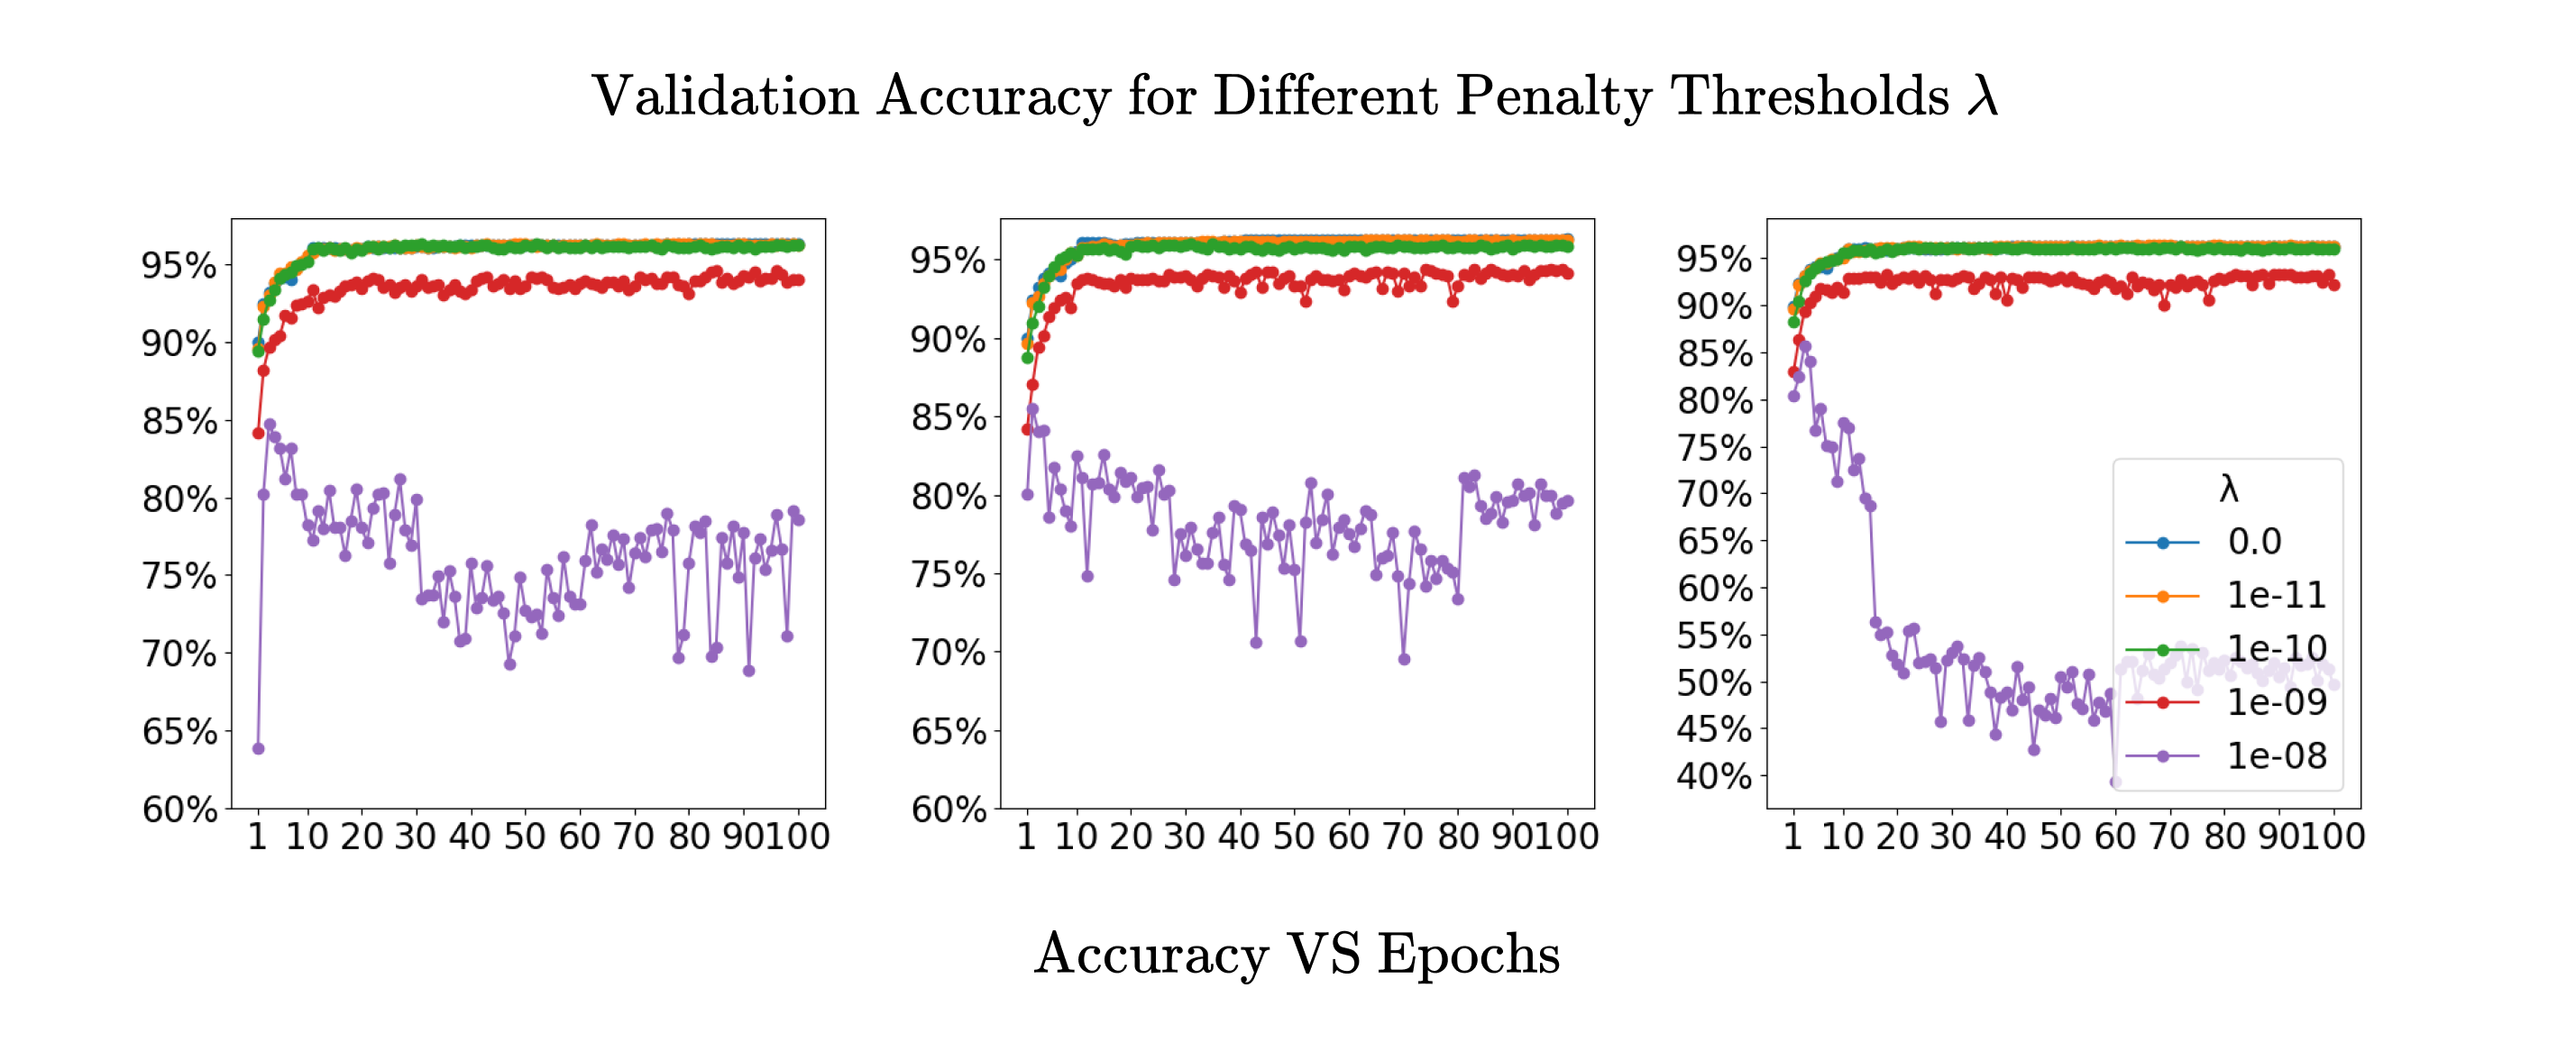
\includegraphics[width=14cm]{val-accs-over-epochs-dense.png}
  \caption{Rowwise (left), columnwise (middle) and scalar (right) scaling factor applied to weights of dense layers, with a scalar scaling factor — to biases.}
  \label{fig:val-accs-over-epochs-dense}
\end{figure}

\begin{figure}[h!]
  \centering
  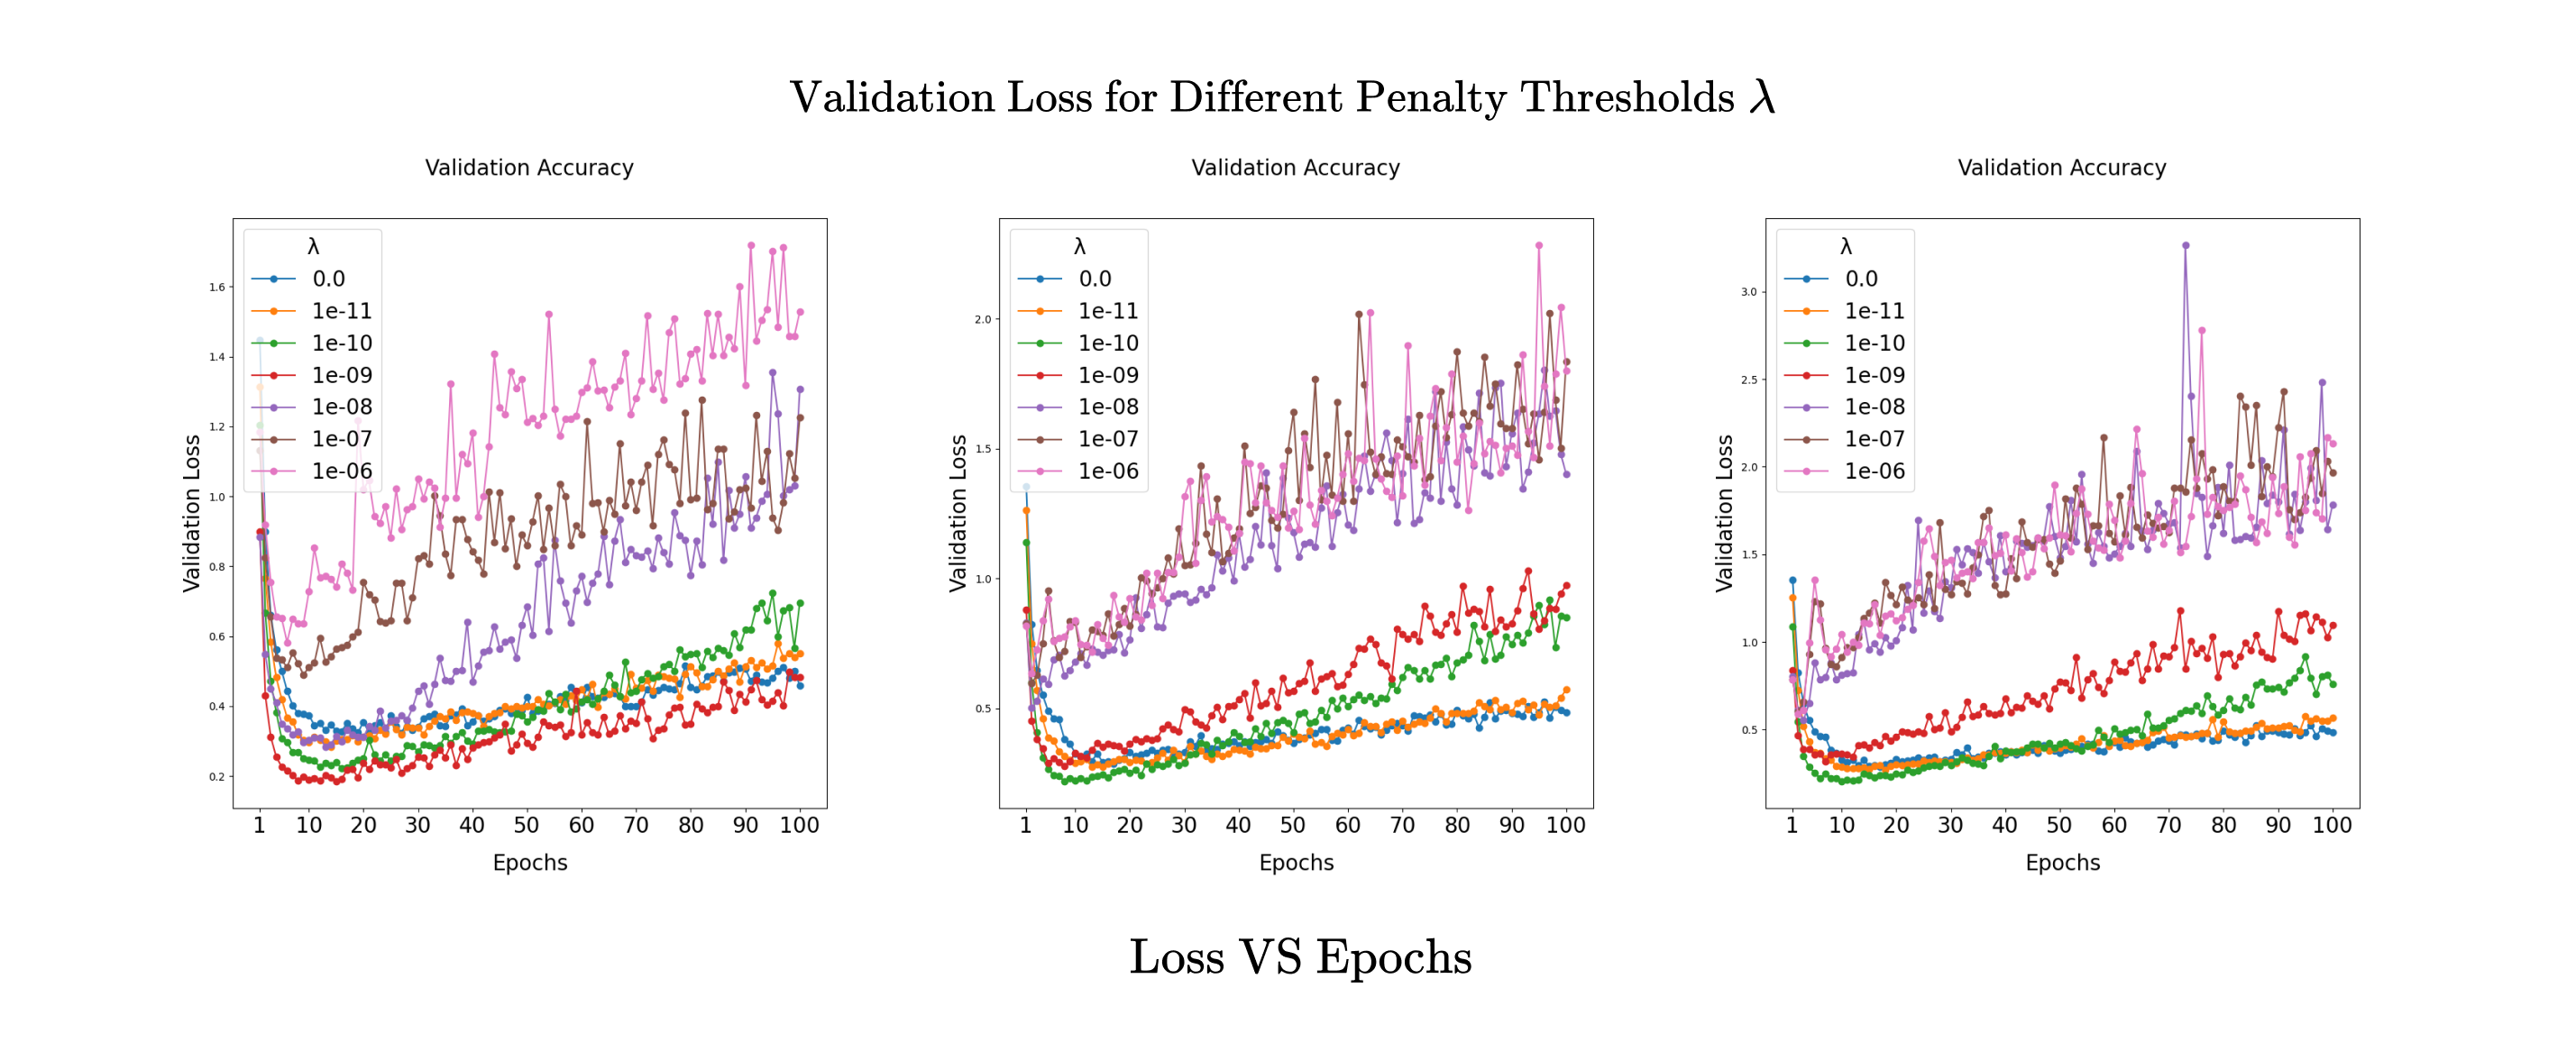
\includegraphics[width=14cm]{val-losses-over-epochs-dense.png}
  \caption{Rowwise (left), columnwise (middle) and scalar (right) scaling factor applied to weights of dense layers, with a scalar scaling factor — to biases.}
  \label{fig:val-losses-over-epochs-dense}
\end{figure}
  
\subsection{Convolutional Layers}
\label{subsec:convolutionallayers}
\hspace*{1em}For the CIFAR-10 dataset, we define a CNN, with six nested convolutional layers. 
Each convolutional layer has a kernel and a bias. We examine four scenarios:
applying the scale factor channel-wise, row-wise, column-wise, and as a single
scalar for the entire kernel. For all scenarios, a scalar factor is used for each 
bias vector, similar to how we quantized dense layers. The configurations are shown in
\cref{tab:scalefactorgranularityconv} for clarity.

\begin{table}[t!]
  \centering
  \scriptsize
  \caption{Scale Factor Granularity for Convolutional Kernels}
  \label{tab:scalefactorgranularityconv}
  \begin{tabular}{lcccc}
    \toprule
    \textbf{Kernel}                      & \textbf{Channel-wise} & \textbf{Row-wise} & \textbf{Column-wise} & \textbf{Scalar} \\ 
    \midrule
    \( K_{1a} \) \( (3, 3, 3, 32) \)     & \( (1, 1, 3, 1) \) & \( (3, 1, 1, 1) \) & \( (1, 3, 1, 1) \) & \( (1, 1, 1, 1) \) \\ 
    \( K_{1b} \) \( (3, 3, 32, 32) \)    & \( (1, 1, 32, 1) \) & \( (3, 1, 1, 1) \) & \( (1, 3, 1, 1) \) & \( (1, 1, 1, 1) \) \\ 
    \( K_{2a} \) \( (3, 3, 32, 64) \)    & \( (1, 1, 32, 1) \) & \( (3, 1, 1, 1) \) & \( (1, 3, 1, 1) \) & \( (1, 1, 1, 1) \) \\ 
    \( K_{2b} \) \( (3, 3, 64, 64) \)    & \( (1, 1, 64, 1) \) & \( (3, 1, 1, 1) \) & \( (1, 3, 1, 1) \) & \( (1, 1, 1, 1) \) \\ 
    \( K_{3a} \) \( (3, 3, 64, 128) \)   & \( (1, 1, 64, 1) \) & \( (3, 1, 1, 1) \) & \( (1, 3, 1, 1) \) & \( (1, 1, 1, 1) \) \\ 
    \( K_{3b} \) \( (3, 3, 128, 128) \)  & \( (1, 1, 128, 1) \) & \( (3, 1, 1, 1) \) & \( (1, 3, 1, 1) \) & \( (1, 1, 1, 1) \) \\ 
    \bottomrule
  \end{tabular}
  \vspace{0.5em}
  \caption*{\footnotesize Note: \( (1, 1, 1, 1) \) denotes a scalar, broadcasted across the kernel for consistency.}
\end{table}

The experiments show that the optimal value for the hyperparameter is \( \lambda = 1e-11\),
across all four scenarios, as depicted in \cref{fig:pareto-cifar-conv}, with 
all scenarios producing approximately the same results.

As an example, the integer values after quantization for the row-wise scenario across all quantized parameters range from \( -22 \) to \( 32 \), 
resulting in \( 60 \) unique values that can be represented with \( \lceil \log_2(60) \rceil = 6 \) bits.

\begin{figure}[b!]
  \centering
  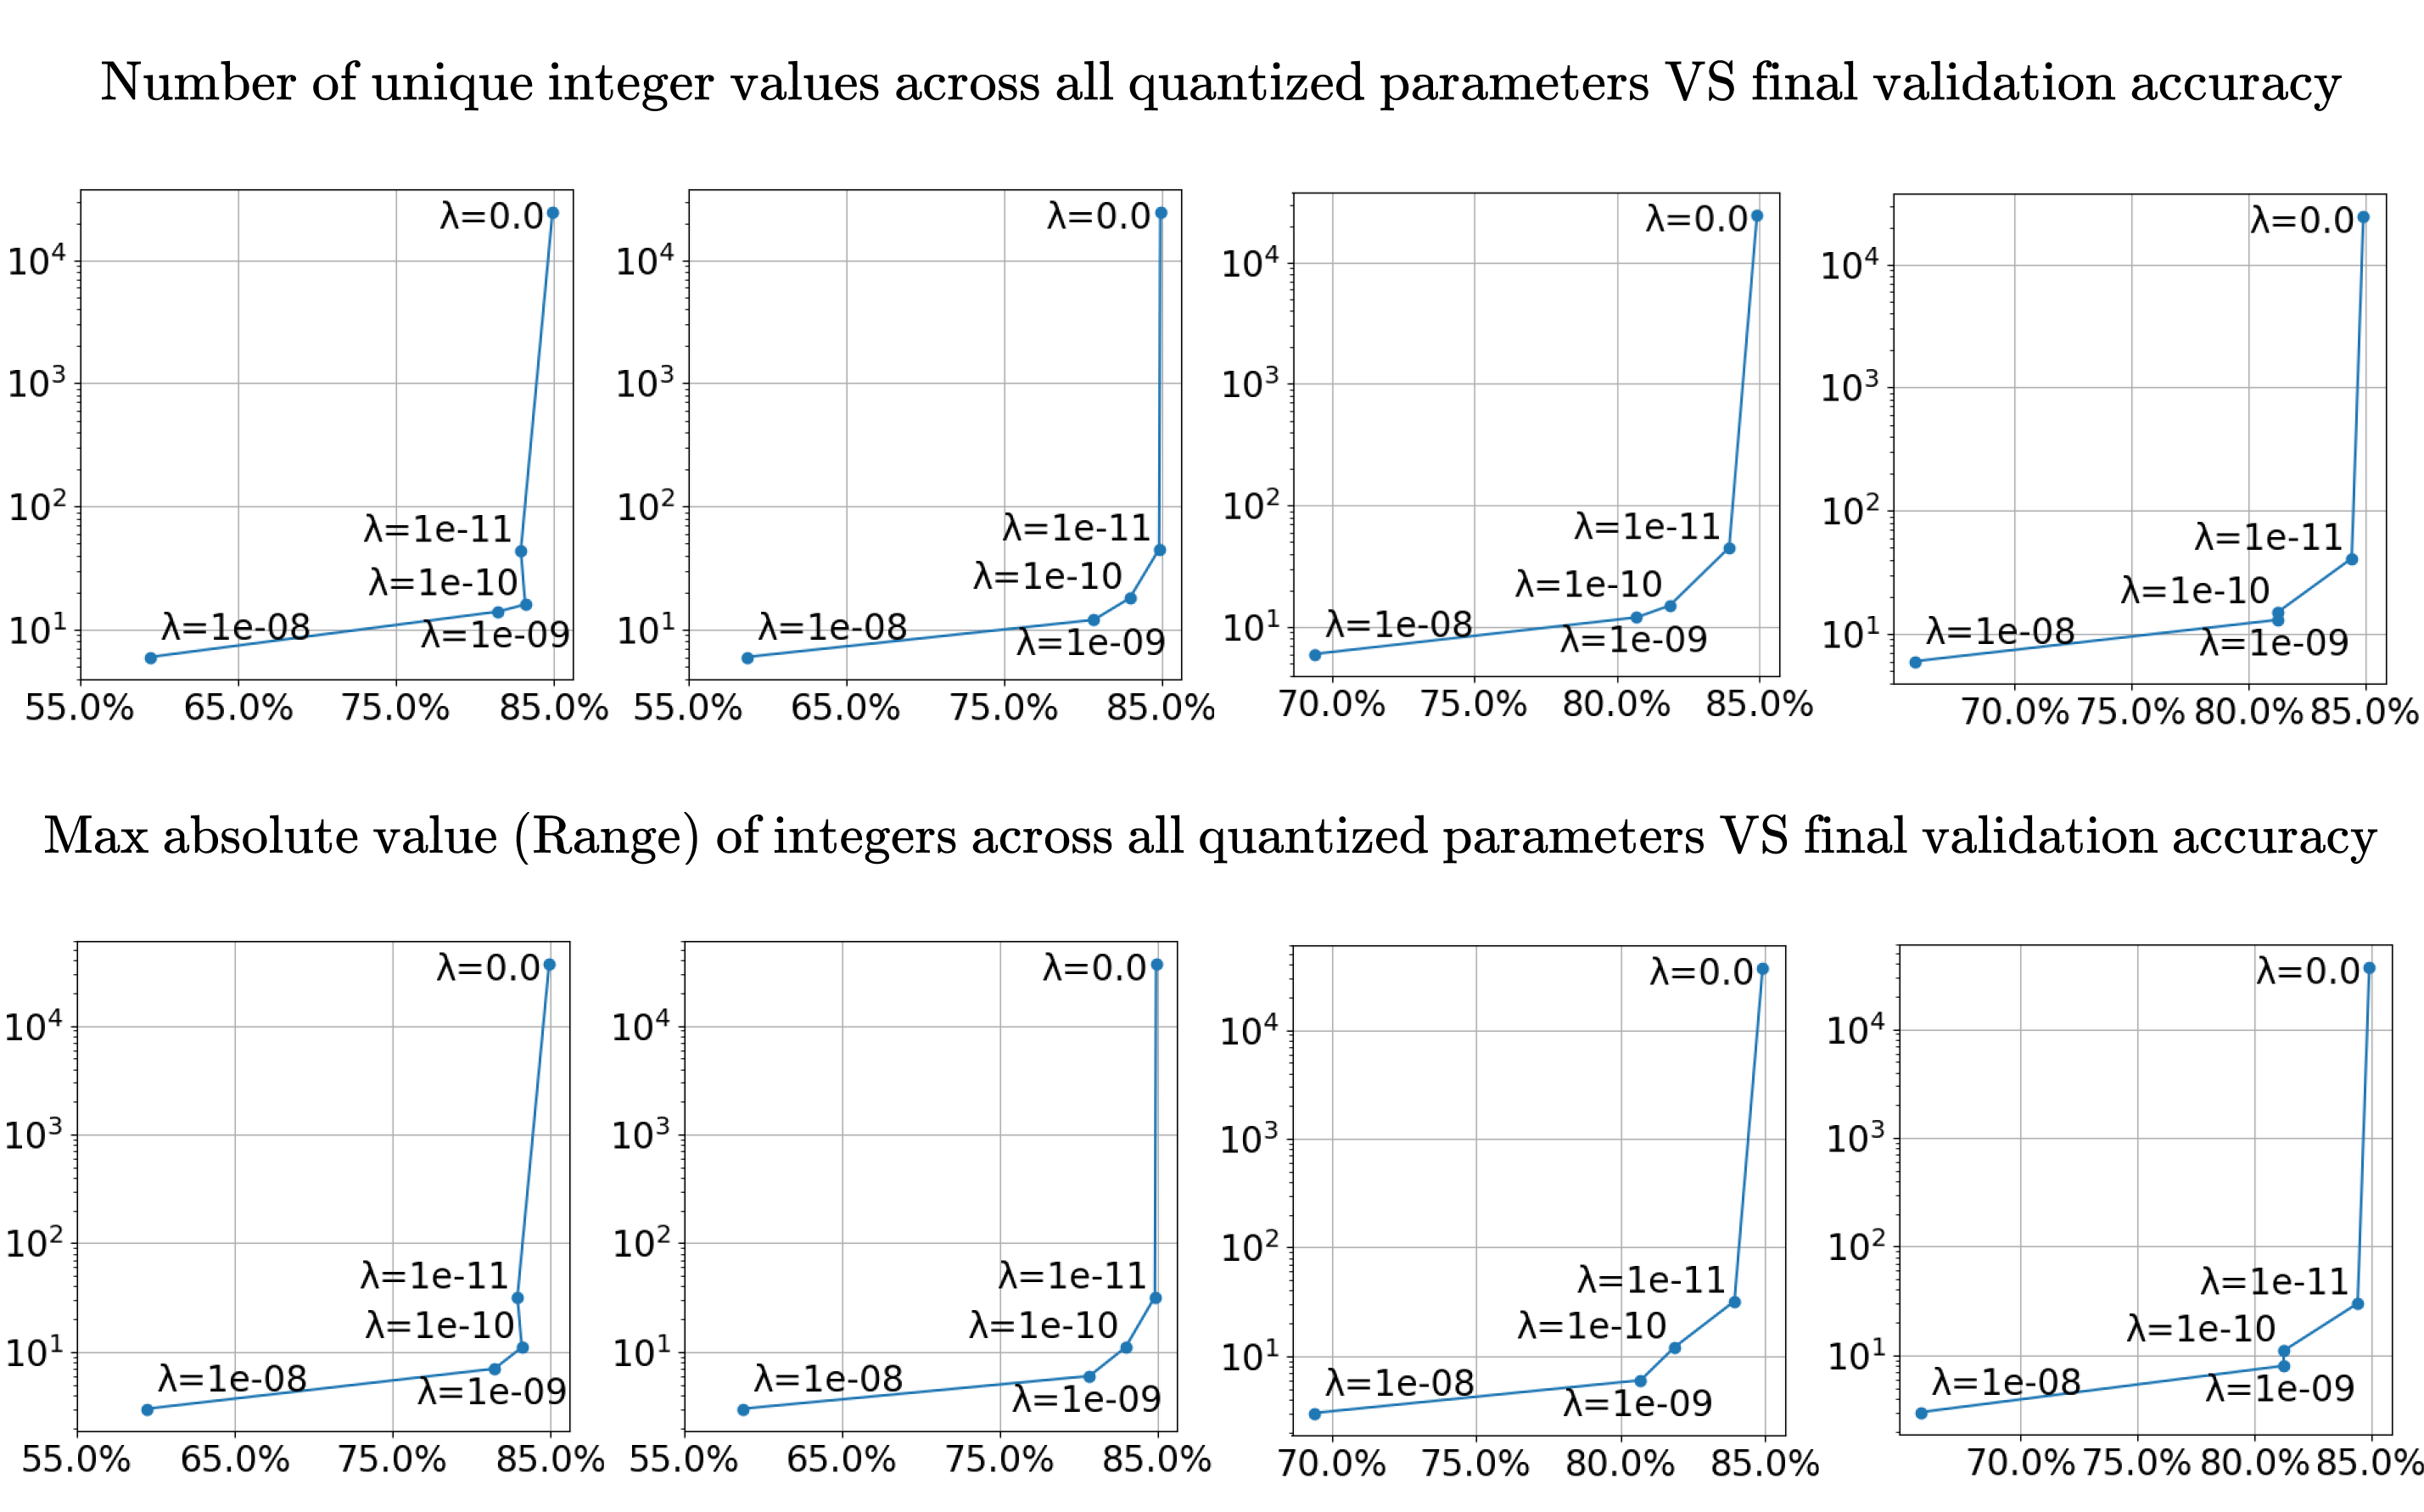
\includegraphics[width=14cm]{pareto-cifar-conv.png}
  \caption{Impact of quantization on accuracy for different \( \lambda \). Channel-wise, row-wise, column-wise and scalar scaling factors applied to kernels of convolutional layers, with a scalar scaling factor — to biases.}
  \label{fig:pareto-cifar-conv}
\end{figure}

Compared to the quantization of dense layers, we notice in \cref{fig:val-losses-over-epochs-conv} that the validation loss 
does not decrease with quantization for \( \lambda = 1e-11 \), which yields the 
best results. Additionally, as evident 
from \cref{fig:val-accs-over-epochs-conv}, the accuracy
degrades slightly, indicating that the quantization process introduces some impact on the model's predictions.
However, the pareto plots in \cref{fig:pareto-cifar-conv} indicate that
there are 

\begin{figure}[t!]
  \centering
  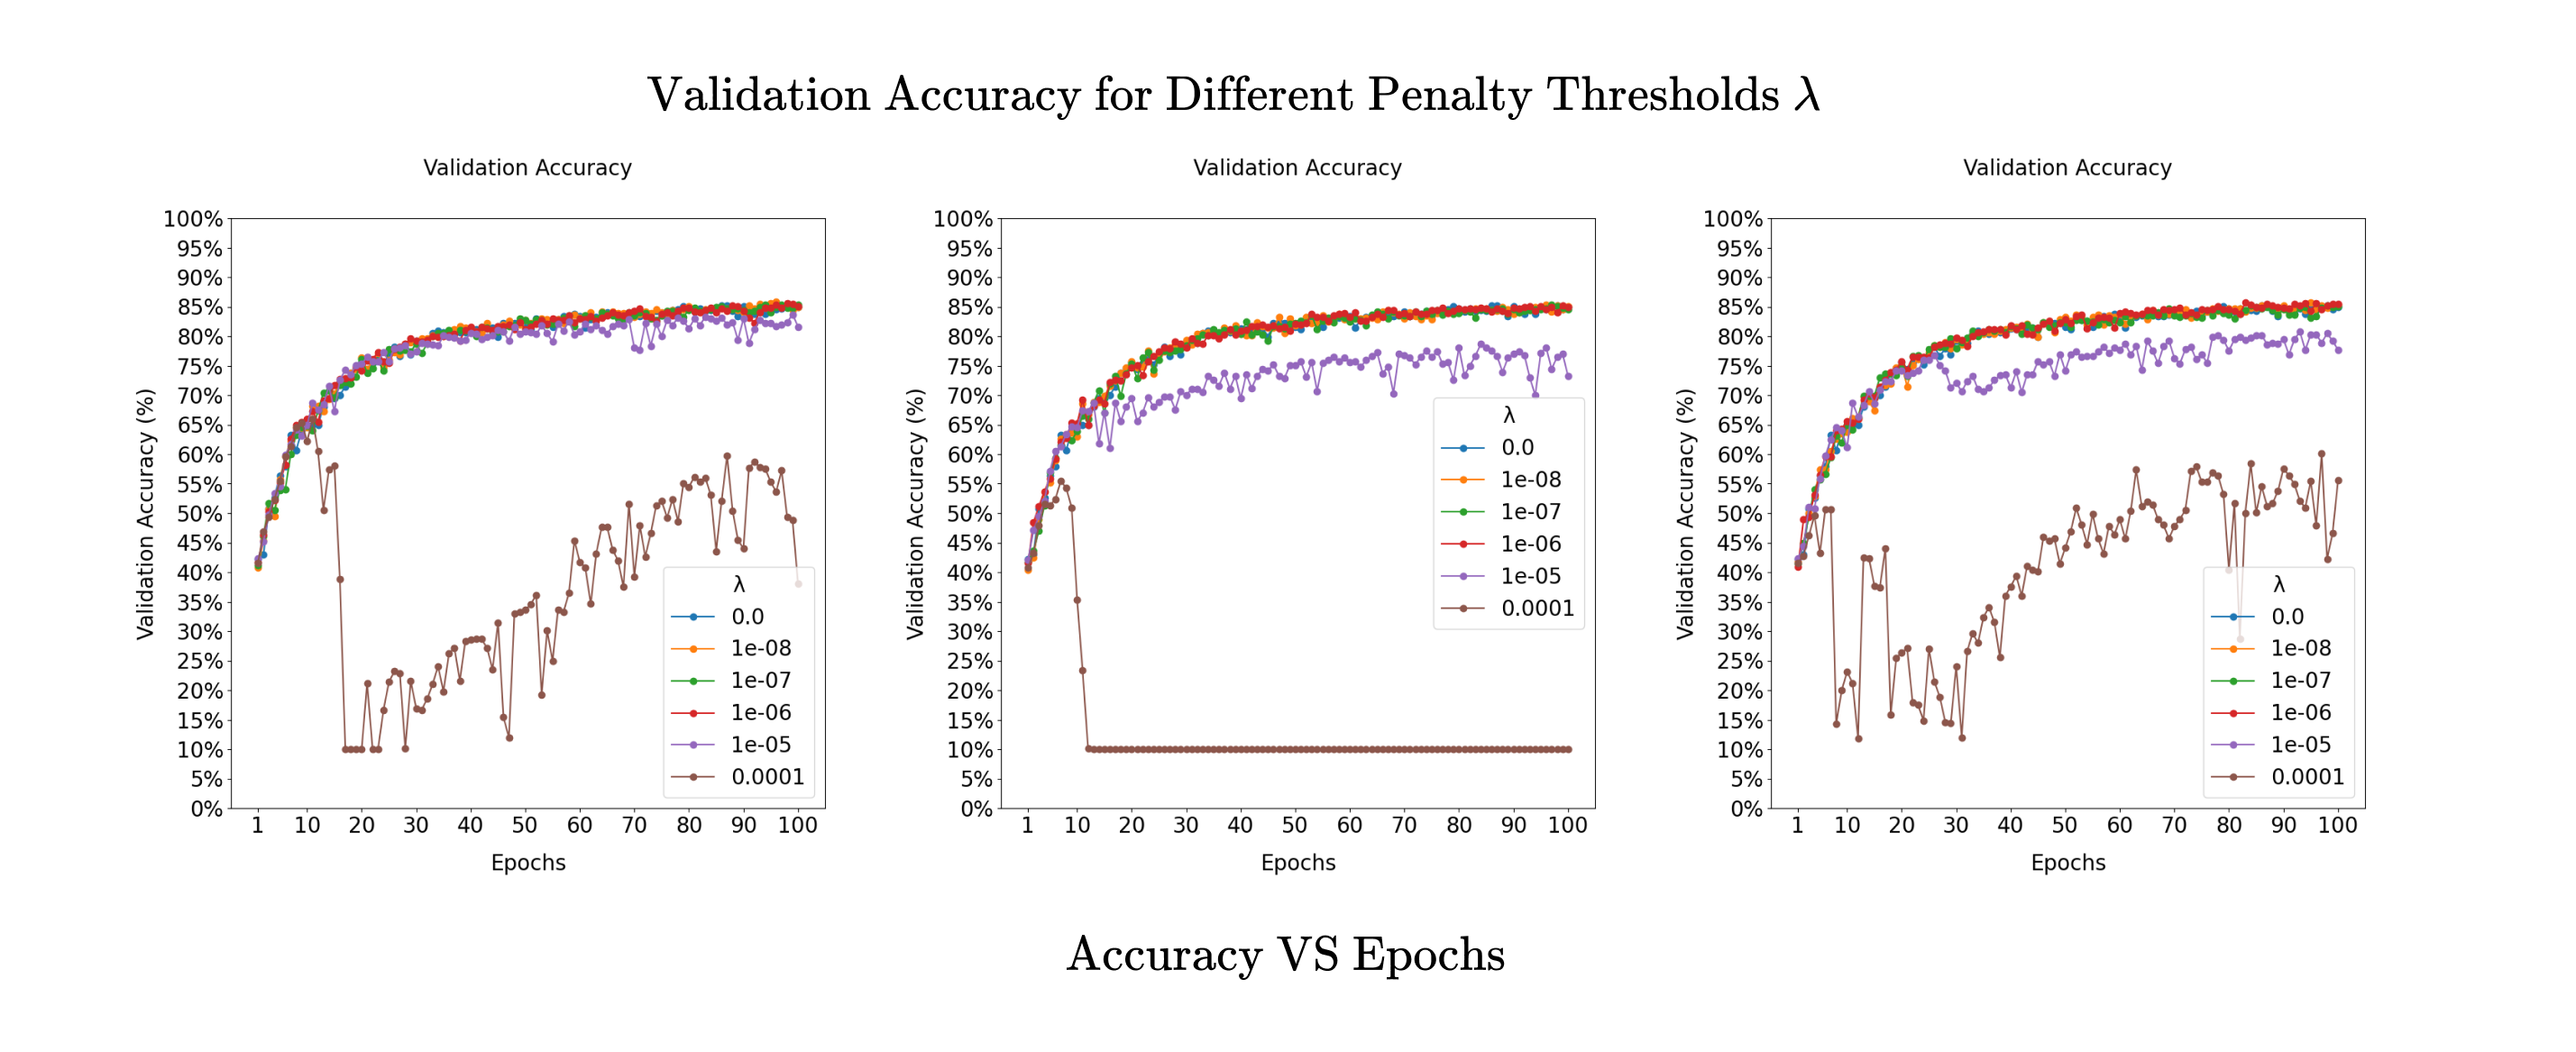
\includegraphics[width=14cm]{val-accs-over-epochs-conv.png}
  \caption{Channel-wise, row-wise, column-wise and scalar scaling factor applied to kernels of convolutional layers, with a scalar scaling factor — to biases.}
  \label{fig:val-accs-over-epochs-conv}
\end{figure}

\begin{figure}[b!]
  \centering
  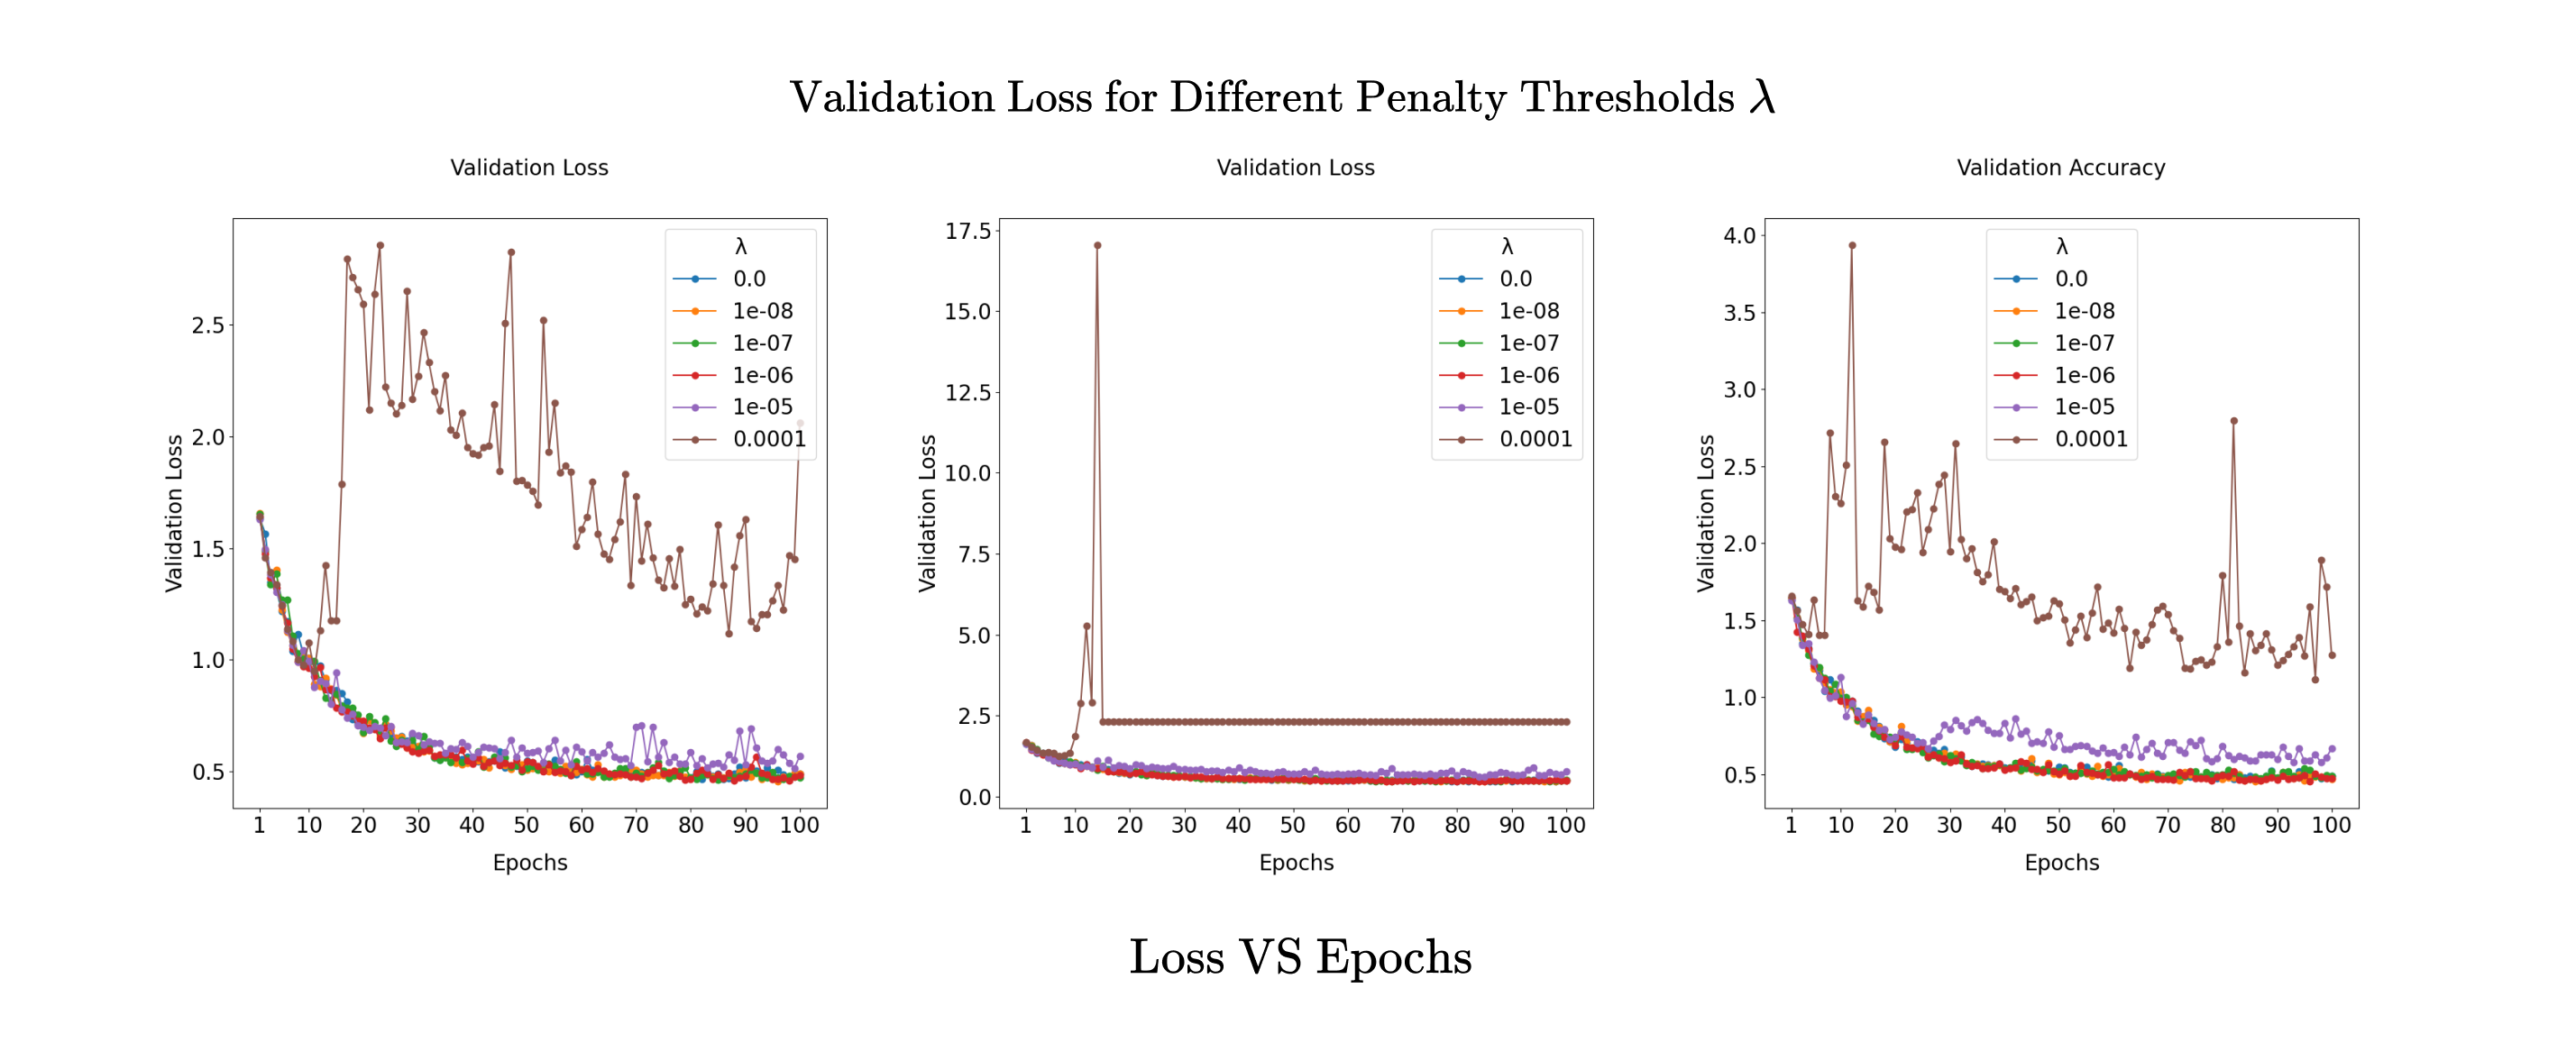
\includegraphics[width=14cm]{val-losses-over-epochs-conv.png}
  \caption{Channel-wise, row-wise, column-wise and scalar scaling factor applied to kernels of convolutional layers, with a scalar scaling factor — to biases.}
  \label{fig:val-losses-over-epochs-conv}
\end{figure}
% ------------------------------------------------------------
% ----------------------- Custom loss terms analysis ----------------------- 
% ------------------------------------------------------------

\section{Systematic Analysis of Custom Loss Terms}
\label{sec:dataset}

